\documentclass{sig-alternate-sigmod09}

\usepackage[hidelinks, bookmarks=true,pdfborder= 0 0 0]{hyperref}

\usepackage{tikz}
\usetikzlibrary{calc,trees,positioning,arrows,chains,shapes.geometric,%
  decorations.pathreplacing,decorations.pathmorphing,shapes,%
  matrix,shapes.symbols,plotmarks,decorations.markings,shadows}

\DeclareMathOperator{\atantwo}{atan2}

\hypersetup{
pdfauthor={Patrick Brosi},
pdfkeywords=,
pdftitle={Metro Maps on Octilinear Grid Graphs},
pdfsubject={},
pdfcreator={},
pdfproducer={}
}

\newcommand\todo[1]{\textcolor{blue}{[TODO: #1]}}
\newcommand\TODO[1]{\textcolor{blue}{\small [TODO: #1]}}

% Input Graph

\def\iG{G}  % Input graph
\def\iV{V}  % Input nodes
\def\iv{v}  % Input node
\def\iE{E}  % Input edges
\def\ie{e}  % Input edge

% Drawing

\newcommand\drawing[1]{\mathcal{D}_{#1}}  % Drawing of graph
\newcommand\initdrawing[1]{\drawing{#1}^*}  % Drawing of graph

\def\drawingcurvesym{c}  % edge curve part of drawing
\def\drawingpossym{p}    % node position part of drawing

\newcommand\drawingcurve[1]{\drawingcurvesym(#1)}  % Drawing curve of argument edge
\newcommand\drawingpos[1]{\drawingpossym(#1)}  % Drawing pos urve of argument node

% Grid

\def\gScale{C}
\def\gmind{\hat d}


% Octilinear grid graph

\def\gG{\Gamma}  % Grid graph
\def\gV{\Psi}  % Grid graph nodes
\def\gv{\psi}  % Grid graph node
\def\gE{\Omega}  % v edges
\def\ge{\omega}  % Grid graph edge

\newcommand\ggv[2]{\gv_{#1, #2}}  % Grid node at #1, #2
\newcommand\gpv[3]{\gv_{#1, #2}^{#3}}  % Port #3 node at #1, #2
\newcommand\gse[3]{\ge_{#1, #2}^{#3}}  % Sink edge #3 node at #1, #2
\newcommand\gbe[4]{\ge_{#1, #2}^{#3, #4}}  % Bend edge for angle #4 at port #3 at node at #1, #2

\def\gPath{p}    % path on grid graph
\def\gPathOcti{p'}    % path on octilinear grid graph

\newcommand\gPturn[1]{c_{#1}}  % Turn penalty
\newcommand\gPturnEdge[1]{c'_{#1}}  % Turn penalty
\def\gHopcost{c_h}    % Hop cost in grid graph
\def\gHopcostOcti{c'_h}    % Hop cost in grid graph
\def\gSinkcost{c_s}    % Hop cost in grid graph
\newcommand\gPcost[1]{c(#1)}  % Path cost
\newcommand\gPcostOcti[1]{c'(#1)}  % Octilinear path cost

% ILP

\newcommand\gvused[2]{x_{#1#2}}	% bin. decision variable whether grid node #1 is assigned to input node #2
\newcommand\geused[2]{x_{#1#2}}	% bin. decision variable whether grid edge #1 is used be input edge #2

\newcommand\dir[2]{\delta_{#1#2}}	% variable telling the direction of edge #2 at node #1
\newcommand\dirdiff[2]{\Delta_{#1#2}}	% variable telling the direction difference of edge #1 and edge #2

\newcommand\bend[3]{\Delta_{#1#2}^{#3}}	% variable telling the direction difference of edge #1 and edge #2

\def\ldeg{\text{ldeg}}

\begin{document}
\title{Metro Maps on Octilinear Grid Graphs}
\subtitle{- sketch -}

\numberofauthors{1}
%\author{Patrick Brosi\\\affaddr{University of Freiburg}\\\affaddr{Chair of Algorithms and Data Structures}}

\maketitle

\section{Abstract}

We investigate a novel approach to the problem of drawing octilinear Metro Maps.
Our approach is based on shortest-path calculations on a specially crafted octilinear grid graph, where edge bends are added to the total cost of the path by means of explicit turn edges.
Our approach can be optimized exactly via an Integer Linear Program (ILP) or approximately by iteratively calculating shortest-paths between node candidates in the octilinear grid graph.
Most importantly, it allows us to revisit earlier work [Stott] which used local search techniques to update node positions until a (local) optimum was found, but where octilinearity was not guaranteed.
By recalculating the shortest-path between an updated node and its neighbors on our octilinear grid graph, we can guarantee octilinearity.
Using this approach, we can calculate metro maps which are very close to optimal in a fraction of a second even for large networks.
%As far as we are aware, our technique is the first non-global approach which guarantees octilinear results.
%Our maps are rendered using previous work and are publicly accessible.

\section{Introduction}

\TODO{Write intro}

\subsection{Problem definition}

Given an undirected planar input graph $\iG = (\iV, \iE)$, where $\iV$ are stations (or other location of interests in a public transit network) and $\iE$ are connections between those stations.
We say $\drawing{\iG} = (\drawingpossym, \drawingcurvesym)$ is a drawing of $\iG$, where $\drawingpos{\iv}$ assigns a position to every node $\iv \in \iV$ and $\drawingcurve{\ie} = (q_0, q_1, ..., q_n)$ assigns a piecewise linear curve to every edge $\ie \in \iE$.
The initial input drawing $\initdrawing{\iG}$ assigns each node a geographical real-world position, and each edge an (optional) real-world trajectory.
\TODO{mention line labels and use same definition as in LOOM paper}
Our goal is to find a schematic drawing $\mathcal{D}'_G$ that resembles a classic Metro Map.
This is usually formalized as a set of hard and soft constraints \cite{nb, ...}.
The hard constraints may be summarized as:
\begin{enumerate}
\setlength\itemsep{.1em}
\item \emph{Octilinearity}. Each edge curve $\drawingcurve{\ie}$ may only consist of segments whose orientation is a multiple of $45^{\circ}$.
\item \emph{Topology preservation}. The input embedding should be respected. In particular, no crossings between edges should be introduced and non-incident edges should never share common points.
\end{enumerate}
Additionally, the following soft constraints are usually employed:
\begin{enumerate}
\setlength\itemsep{.1em}
\item \emph{Edge monotony}. The number of edge bends should be minimized and large angles preferred.
\item \emph{Geographical accuracy}. The original node positions should be changed as little as possible.
\item \emph{Map density}. There should be a minimum distance $\gmind$ between the anchor points of curves to ensure readability.
\end{enumerate}

With respect to edge monotony and octilineary, previous work often defined the problem as finding an octilinear embedding of the input graph, where each edge is represented by a straight octilinear arc.
We use a slightly different approach and state the problem as finding the optimal posititions $p(v) \in \mathbb{N}^2$ on a grid for each station node and curves $c(e) = (q_0, q_1, ..., q_n)$, $q_i \in \mathbb{N}^2$ connecting them. 
Most importantly, for two suceeding points $q_i = (x_i, y_i)$ and $q_{i+1} = (x_{i+1}, y_{i+1})$, we require that they have a distance of 1 with respect to the uniform norm $L^{\infty}$.
This means that the distance $|q_{i+1} - q_{i}|_{\infty}$ between them is defined as $\max \{|x_{i+1} - x_i|, |y_{i+1} - y_i|\}$.
For any point on the grid, the distance to all its 8 direct neighbors is thus 1.

To project this grid onto a map plane, we use a scale factor $\gScale$, which is essentially the height and length of a grid cell.
If $\gScale$ is set to $\gmind$, a minimum distance between any two grid points is guaranteed to be greater or equal to $\gmind$.

\subsection{Related Work}

Survey Noellenburg %http://i11www.iti.kit.edu/extra/publications/n-asamm-14.pdf
Survey Wolff %http://www1.pub.informatik.uni-wuerzburg.de/pub/wolff/pub/w-dsms-07.pdf
Hong et al., force-based approach
Stott's PhD
steiner trees! %https://www.researchgate.net/profile/Matthias_Mueller-Hannemann/publication/225160153_Approximation_of_Octilinear_Steiner_Trees_Constrained_by_Hard_and_Soft_Obstacles/links/0912f50cf248ec1193000000/Approximation-of-Octilinear-Steiner-Trees-Constrained-by-Hard-and-Soft-Obstacles.pdf

\section{Octilinear Grid Graph}

\begin{figure*}[t]
  \centering
	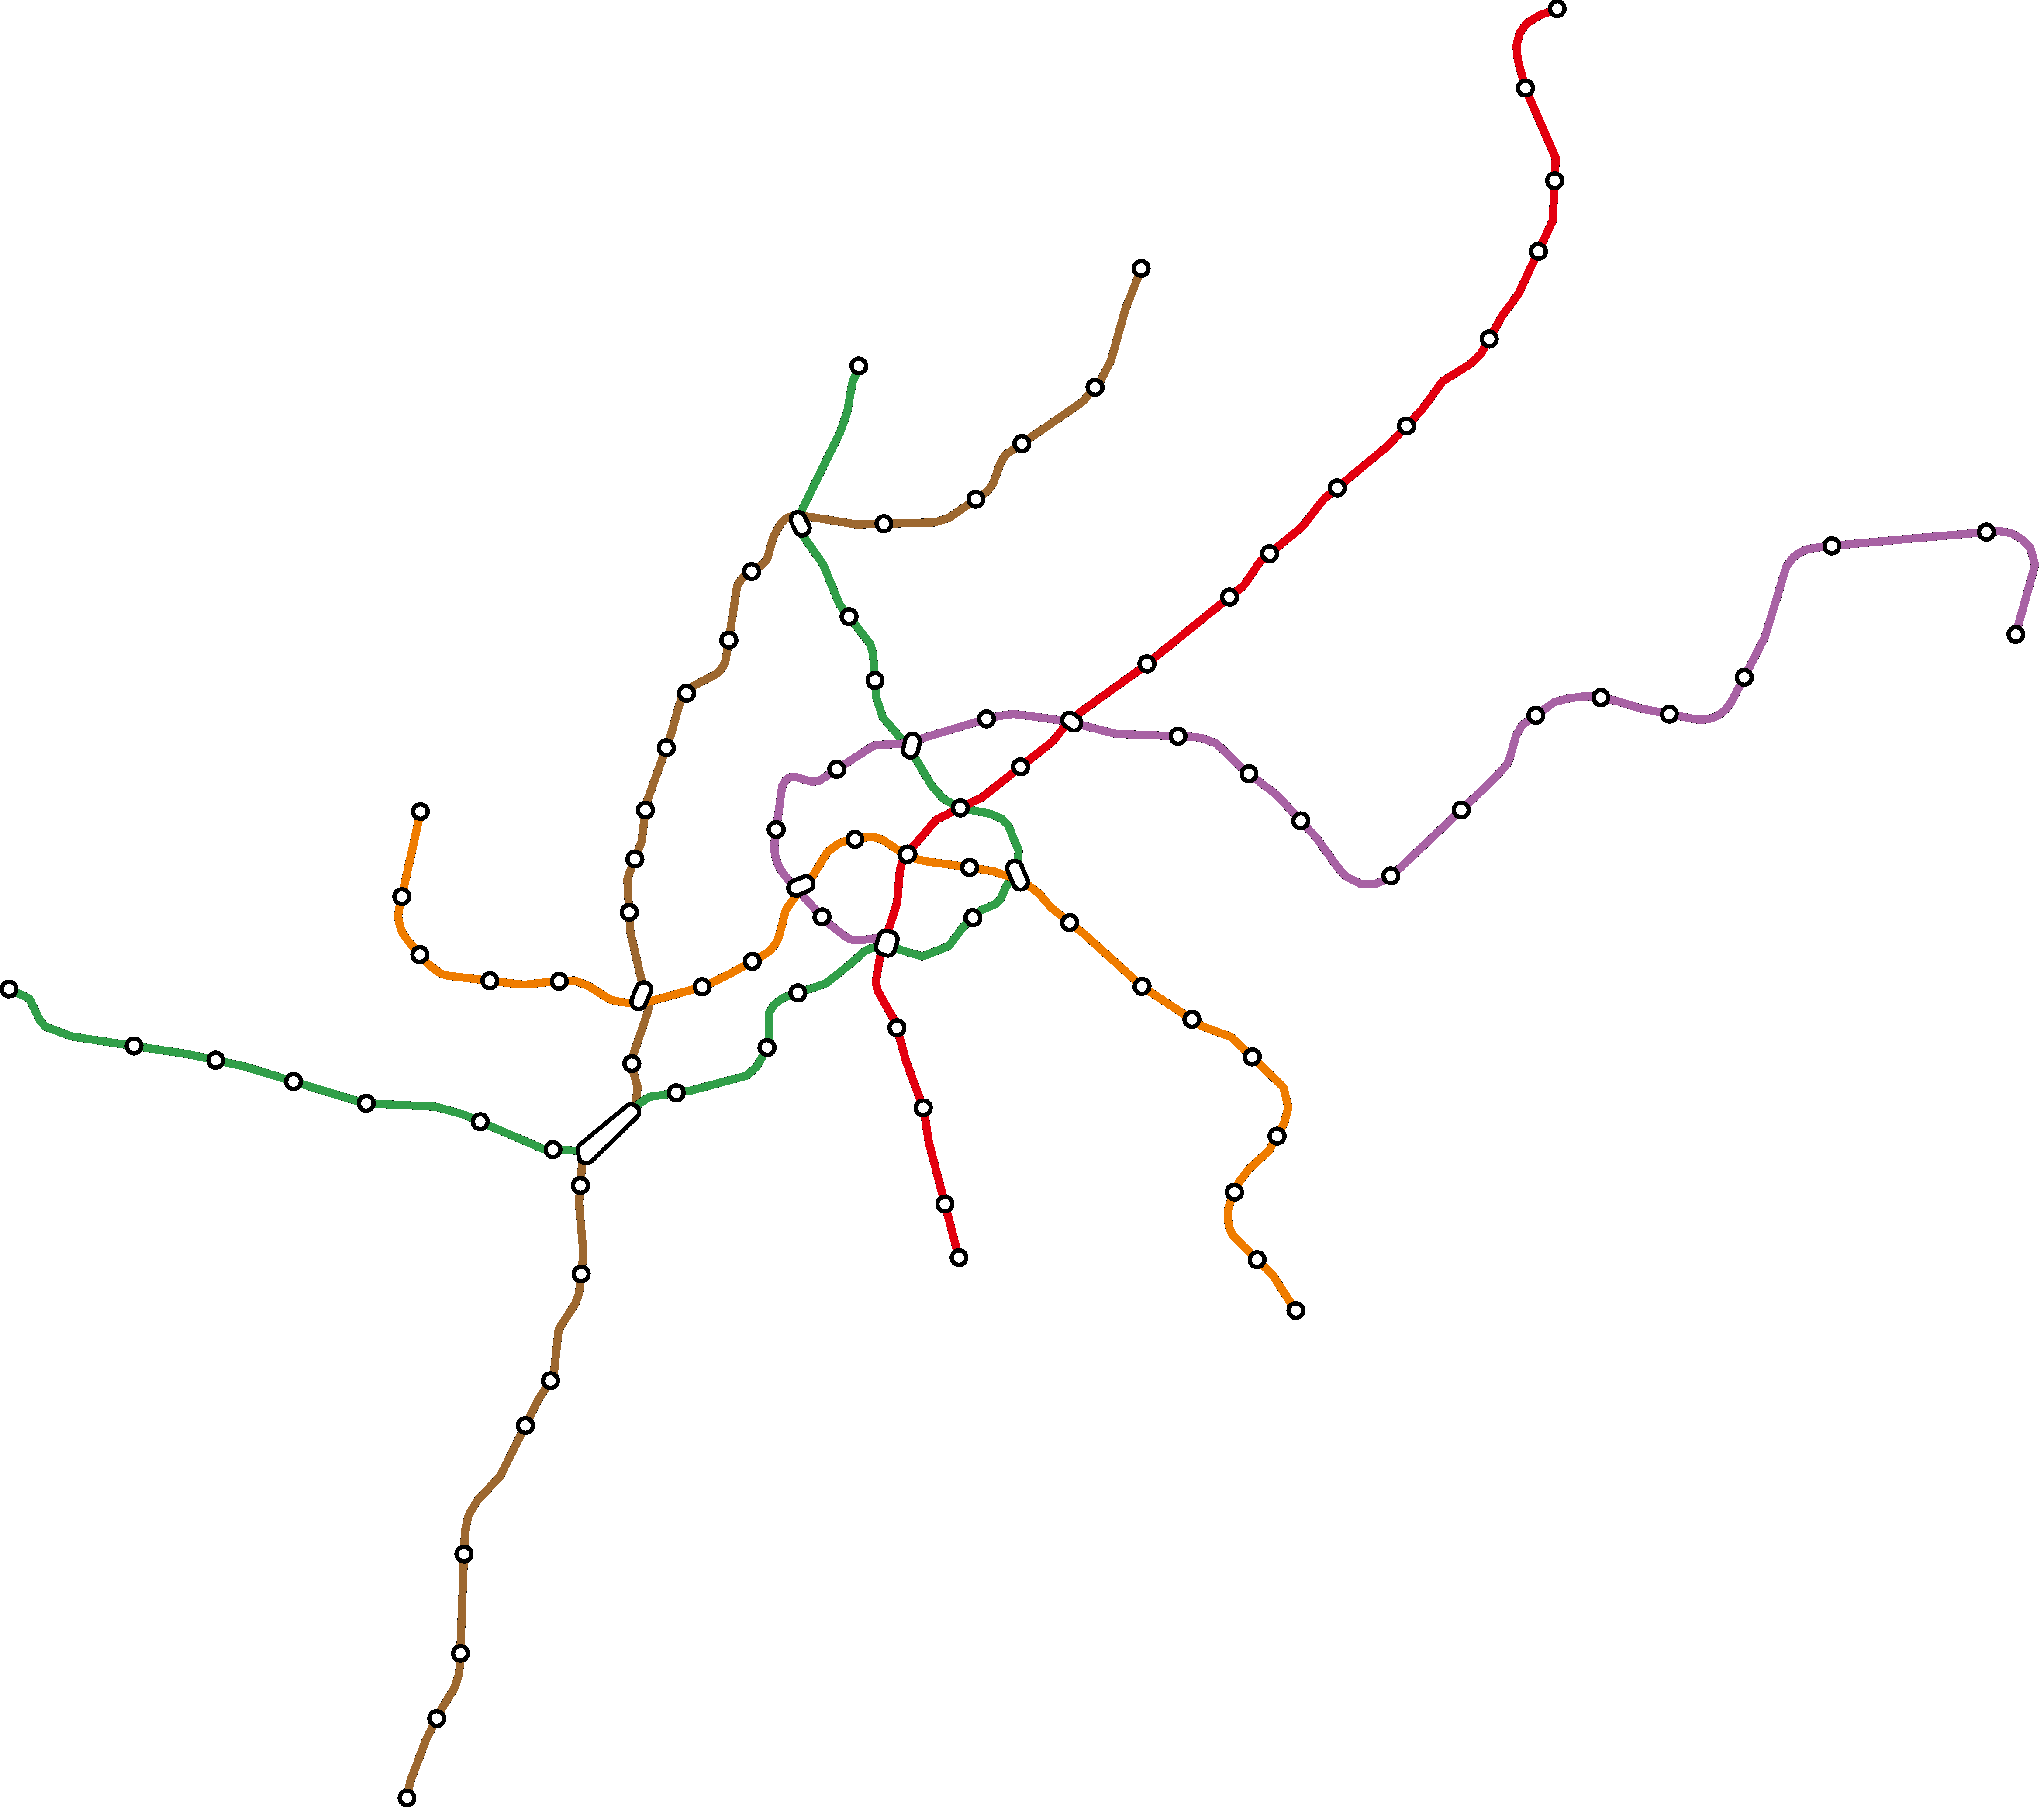
\includegraphics[width=0.474\textwidth]{figures/octi_input.pdf}
	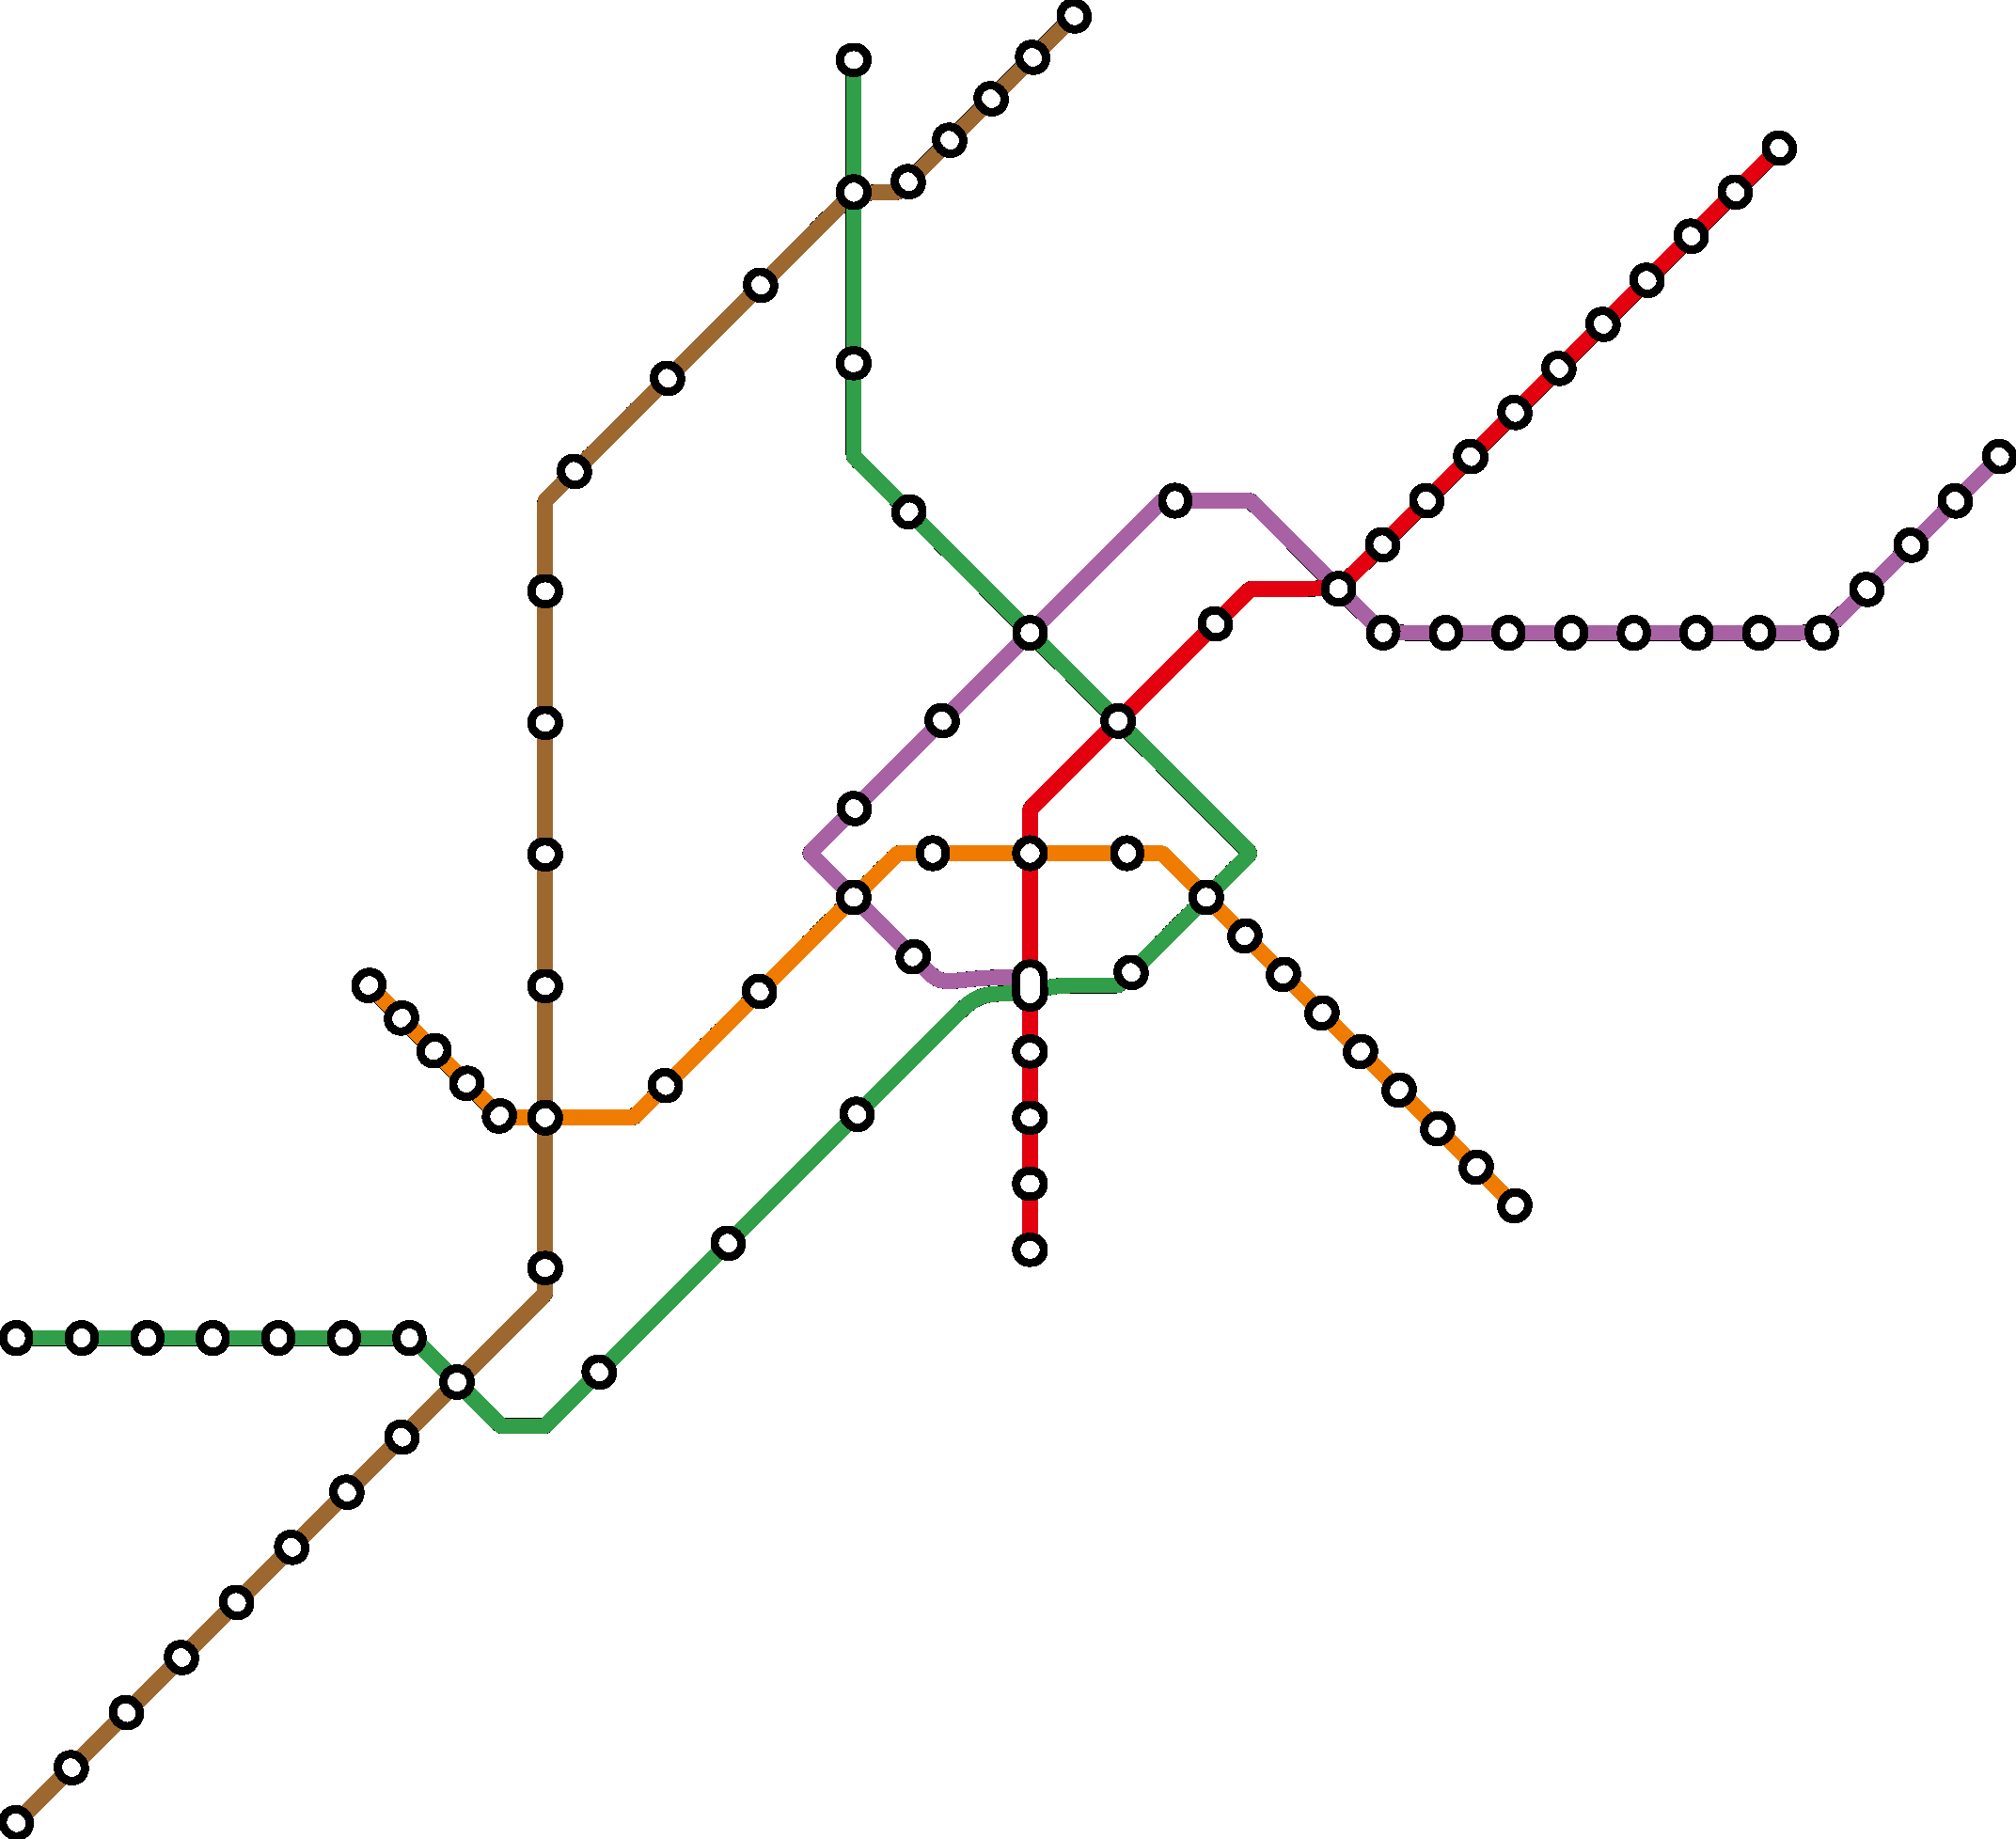
\includegraphics[width=0.474\textwidth]{figures/octi.pdf}
	\caption{The subway network of Vienna, rendered with our approach from raw timetable (GTFS) data (including stop positions).}
	\label{FIG:examplewien}
\end{figure*}

We use an auxiliary undirected graph $\gG = (\gV, \gE)$, where $\gV$ is the set of nodes and $\gE$ is the set of edges and in which every possible path $\gPath = (\gv_0, \gv_1, ..., \gv_n), \gv_i \in \gV$ with $\gv_0 \neq \gv_n$ and $|\gPath| > 1$ represents an octilinear curve with cost $\gPcost{\gPath} = (n - 1) \cdot \gHopcost$, where $\gHopcost$ is the ``hop'' cost of using a single edge.
The graph in Fig.~\ref{FIG:gridgraph},~left trivially satisfies this: we define a $X\times Y$ grid and add nodes $\ggv{x}{y}$ for every grid point.
Each node $\psi_{x,y}$ is connected with its 8 direct neighbors (except at the grid boundaries) $N^0(\ggv{x}{y}) ... N^7(\ggv{x}{y})$, where $N^0(\ggv{x}{y})$ is the ``north'' neighbor of $\ggv{x}{y}$, $N^1(\ggv{x}{y})$ the ``north-east'' neighbor etc..

\subsection{Penalizing Line Bends}

To later be able to optimize soft constraint (1), we additionally want the total cost for a path in $\Gamma$ to reflect the number and accuteness of bends.
The penalty for a turn should be weighted by its degree - either $135^{\circ}$, $90^{\circ}$ or $45^{\circ}$.
We call these penalties $\gPturn{135}$, $\gPturn{90}$ and $\gPturn{45}$.
A straight pass through a node should go unpunished, so $\gPturn{180} = 0$.
Since we aim for a ``smooth'' path through $\gG$ and want to favor obtuse angles, we require $\gPturn{180} \leq \gPturn{135} \leq \gPturn{90} \leq \gPturn{45}$.

We extend our cost function and now search for the path $\gPath = (\gv_0, \gv_1, ..., \gv_i, ..., \gv_n)$ which minimizes
\begin{align}
	\gPcost{\gPath} = (n - 1) \cdot \gHopcost + \sum_{i=1}^{n - 1} t(\gv_{i-1}, \gv_{i+1}),
\end{align}
where $t(\gv_{i-1}, \gv_{i+1})$ is the angular turn cost between edges $\{\gv_{i-1}, \gv_{i}\}$ and $\{\gv_{i}, \gv_{i=1}\}$, that is, either 0, $\gPturn{135}$, $\gPturn{90}$ or $\gPturn{45}$.

\begin{figure}[t]
  \centering
	$\vcenter{\hbox{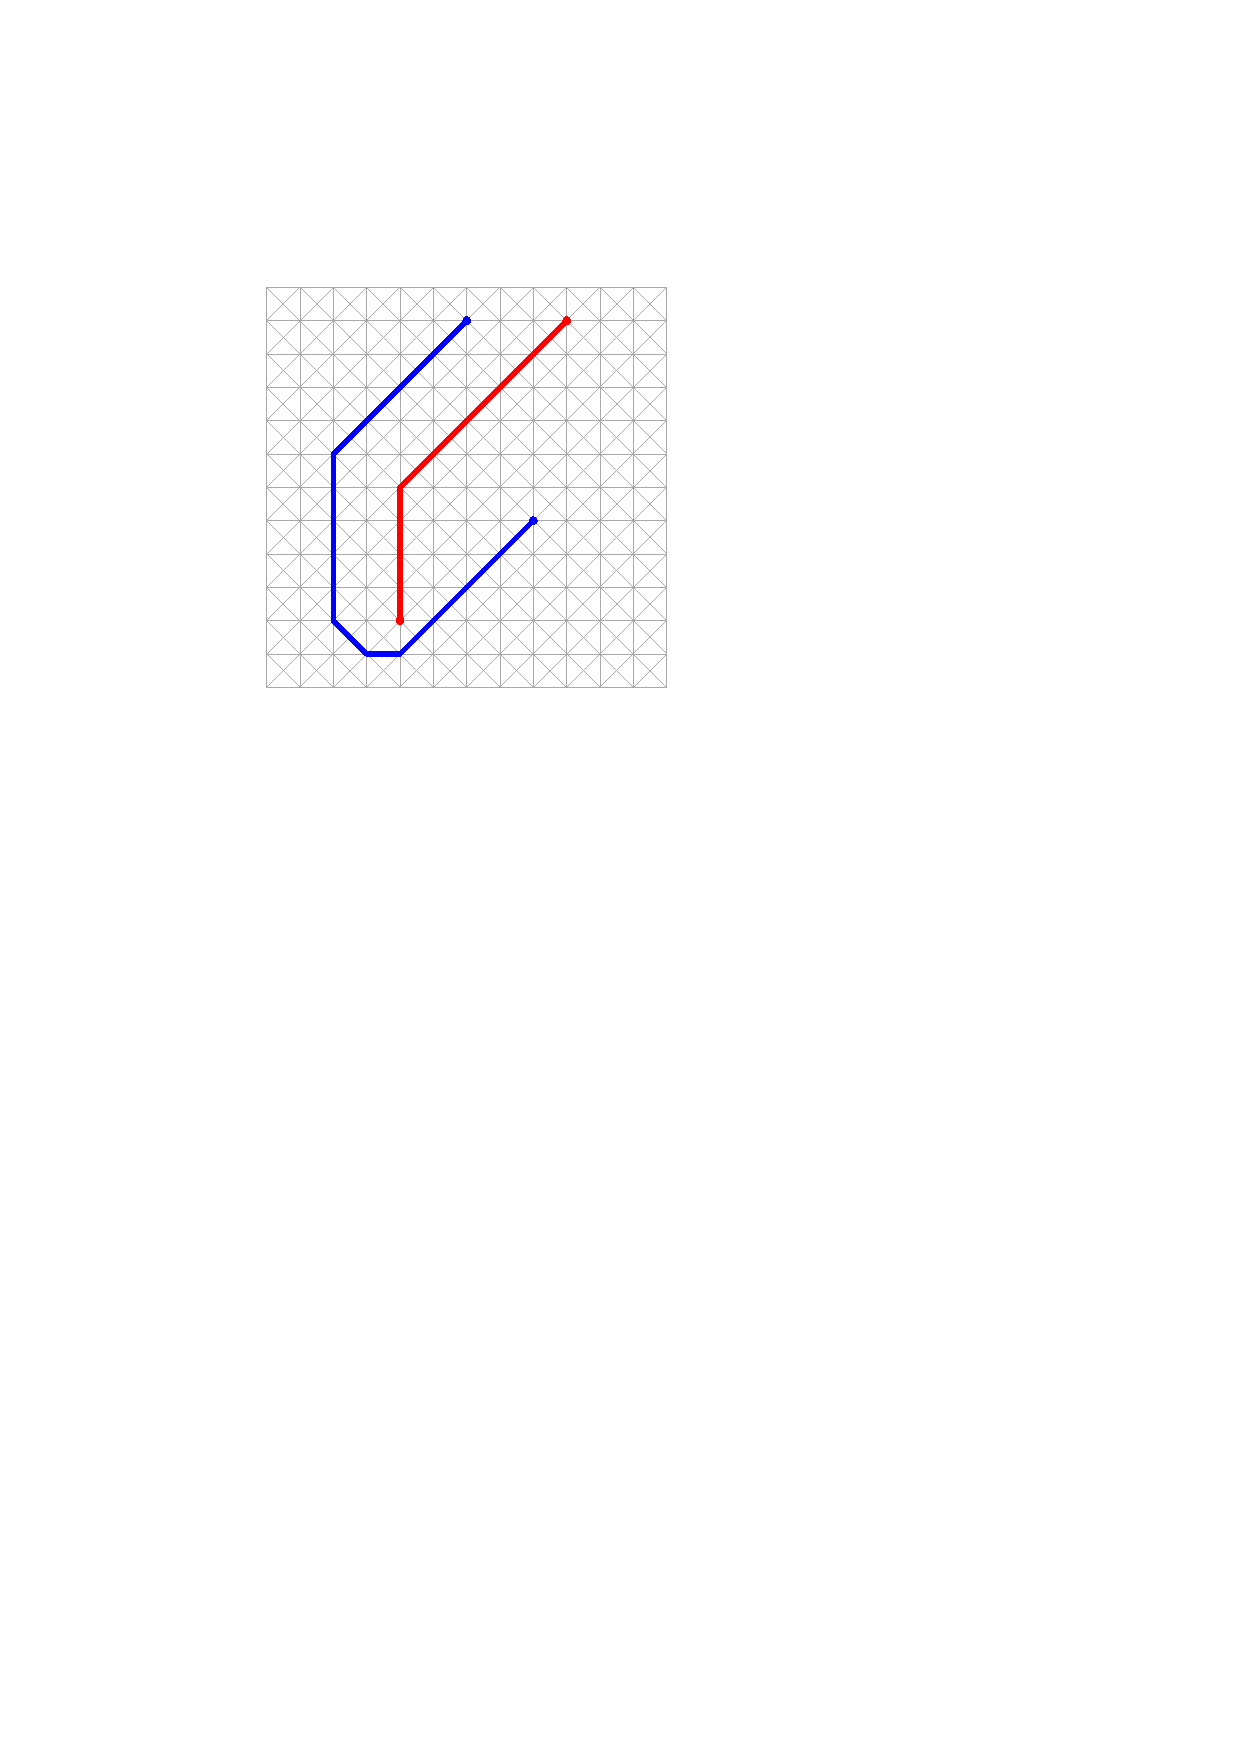
\includegraphics[width=0.474\textwidth]{figures/grid.pdf}}}$
	\caption{Left: A shortest path between $t$ and $u$ on a grid graph with uniform edge cost. Path bends are not minimized. Right: Two shortest path between $(t, u)$, and $(v, w)$ on our octilinear grid graph with uniform grid edge cost $1$ and additional path turn penalties $\gPturn{135} = 1$, $\gPturn{90} = 1.5$ and $\gPturn{45} = 2$. Path $(t, u)$ acts as an obstacle for $(v, w)$.}
	\label{FIG:grids}
\end{figure}

We model this by adding 8 auxiliary port nodes $\gpv{x}{y}{0} ... \gpv{x}{y}{7}$ to every grid node (Fig.~\ref{FIG:gridgraph}).
Each port again corresponds to an outgoing angle in clockwise fashion and is connected to $\ggv{x}{y}$ via sink edges $\gse{x}{y}{0} ... \gse{x}{y}{7}$.
These sink edges allow us to leave from and arrive at an original node $\gv{x}{y}$.
For paths passing through the original grid node $\ggv{x}{y}$, we connect each port $\gpv{x}{y}{i}$ with its 7 - i succeeding (in clockwise fashion) sibling ports with bend edges $\gbe{x}{y}{i}{45}$, $\gbe{x}{y}{i}{90}$, and so forth.

\begin{figure}[h]
  \centering
	$\vcenter{\hbox{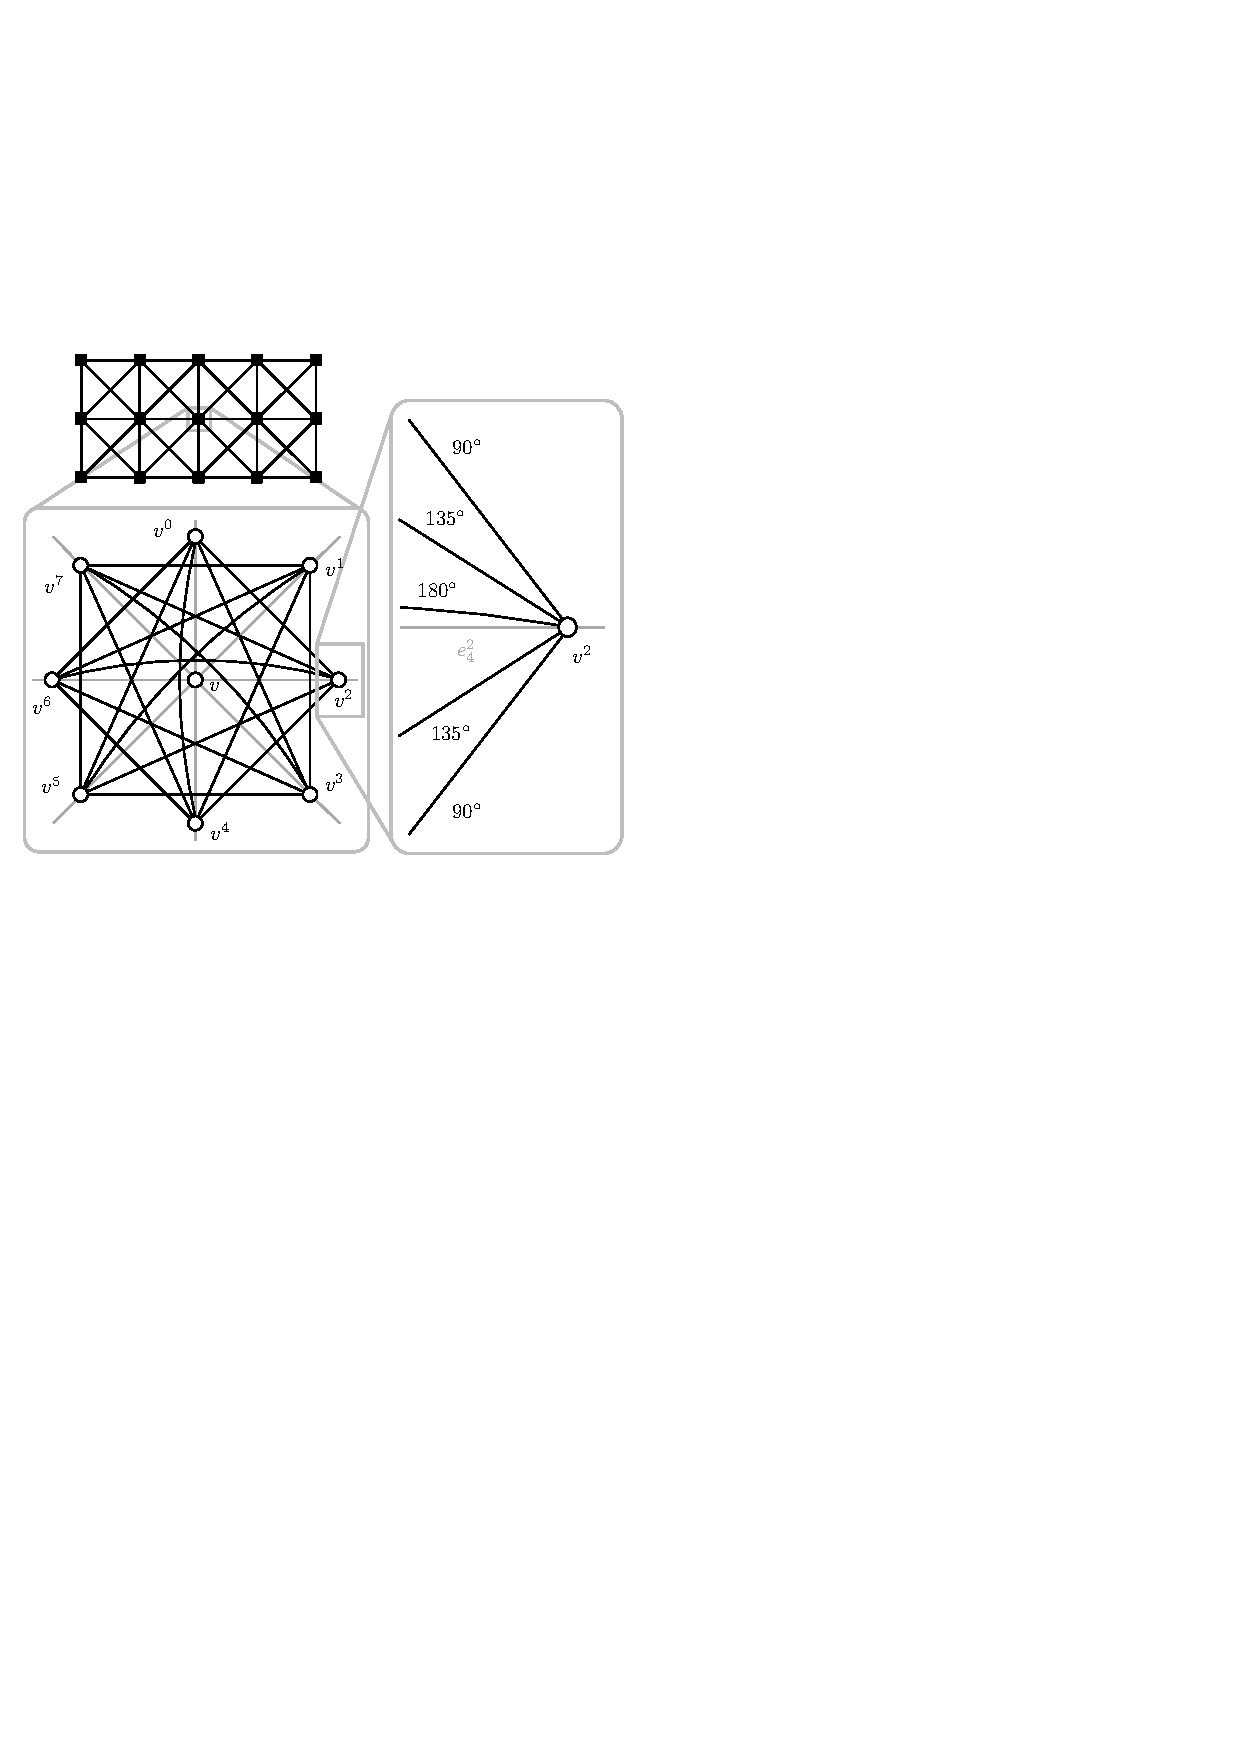
\includegraphics[width=0.45\textwidth]{figures/node.pdf}}}$
	\caption{A $3\times5$ octilinear grid graph. Each node $\psi_i$ has 8 ports $\gv_i^0 ... \gv_i^7$ which are connected to $\gv_i$ by a direct edge. Each port is additionally connected to its $180^{\circ}$, $135^{\circ}$ and $35^{\circ}$ neighbor ports.}
	\label{FIG:gridgraph}
\end{figure}

To be able to distinguish the different node and edge types, we define the set of original grid nodes as $\gV^g \ni \ggv{x}{y}$, the set of port nodes as $\gV^p \ni \gpv{x}{y}{i}$, the set of bend edges as $\gE^b \ni \gbe{x}{y}{i}{\theta}$, the set of sink edges as $\gE^s \ni \gse{x}{y}{i}$ and the set of original grid edges as $\gE^g$.
Note that $\gV = \gV^g \cup \gV^p$ and $\gE = \gE^t \cup \gE^s \cup \gE^g$.

Additionally, for each $\gv \in \gV$, we define $\gv^* \in \gV^g$ as the original grid node belonging to $\gv$ (this may be $\gv$ itself).

As we want to prevent the use of sink edges in pass-through nodes, we set a uniform sink edge cost $\gSinkcost$ high enough so that a sink edge is always more expensive than a turn edge. 
In a shortest path from $s$ to $t$, the only sink edges are then a leaving sink edge adjacent to $s$ and an arriving sink edge adjacent to $t$.

\subsection{Modelling Edge Costs}

\begin{figure*}
  \centering
	$\vcenter{\hbox{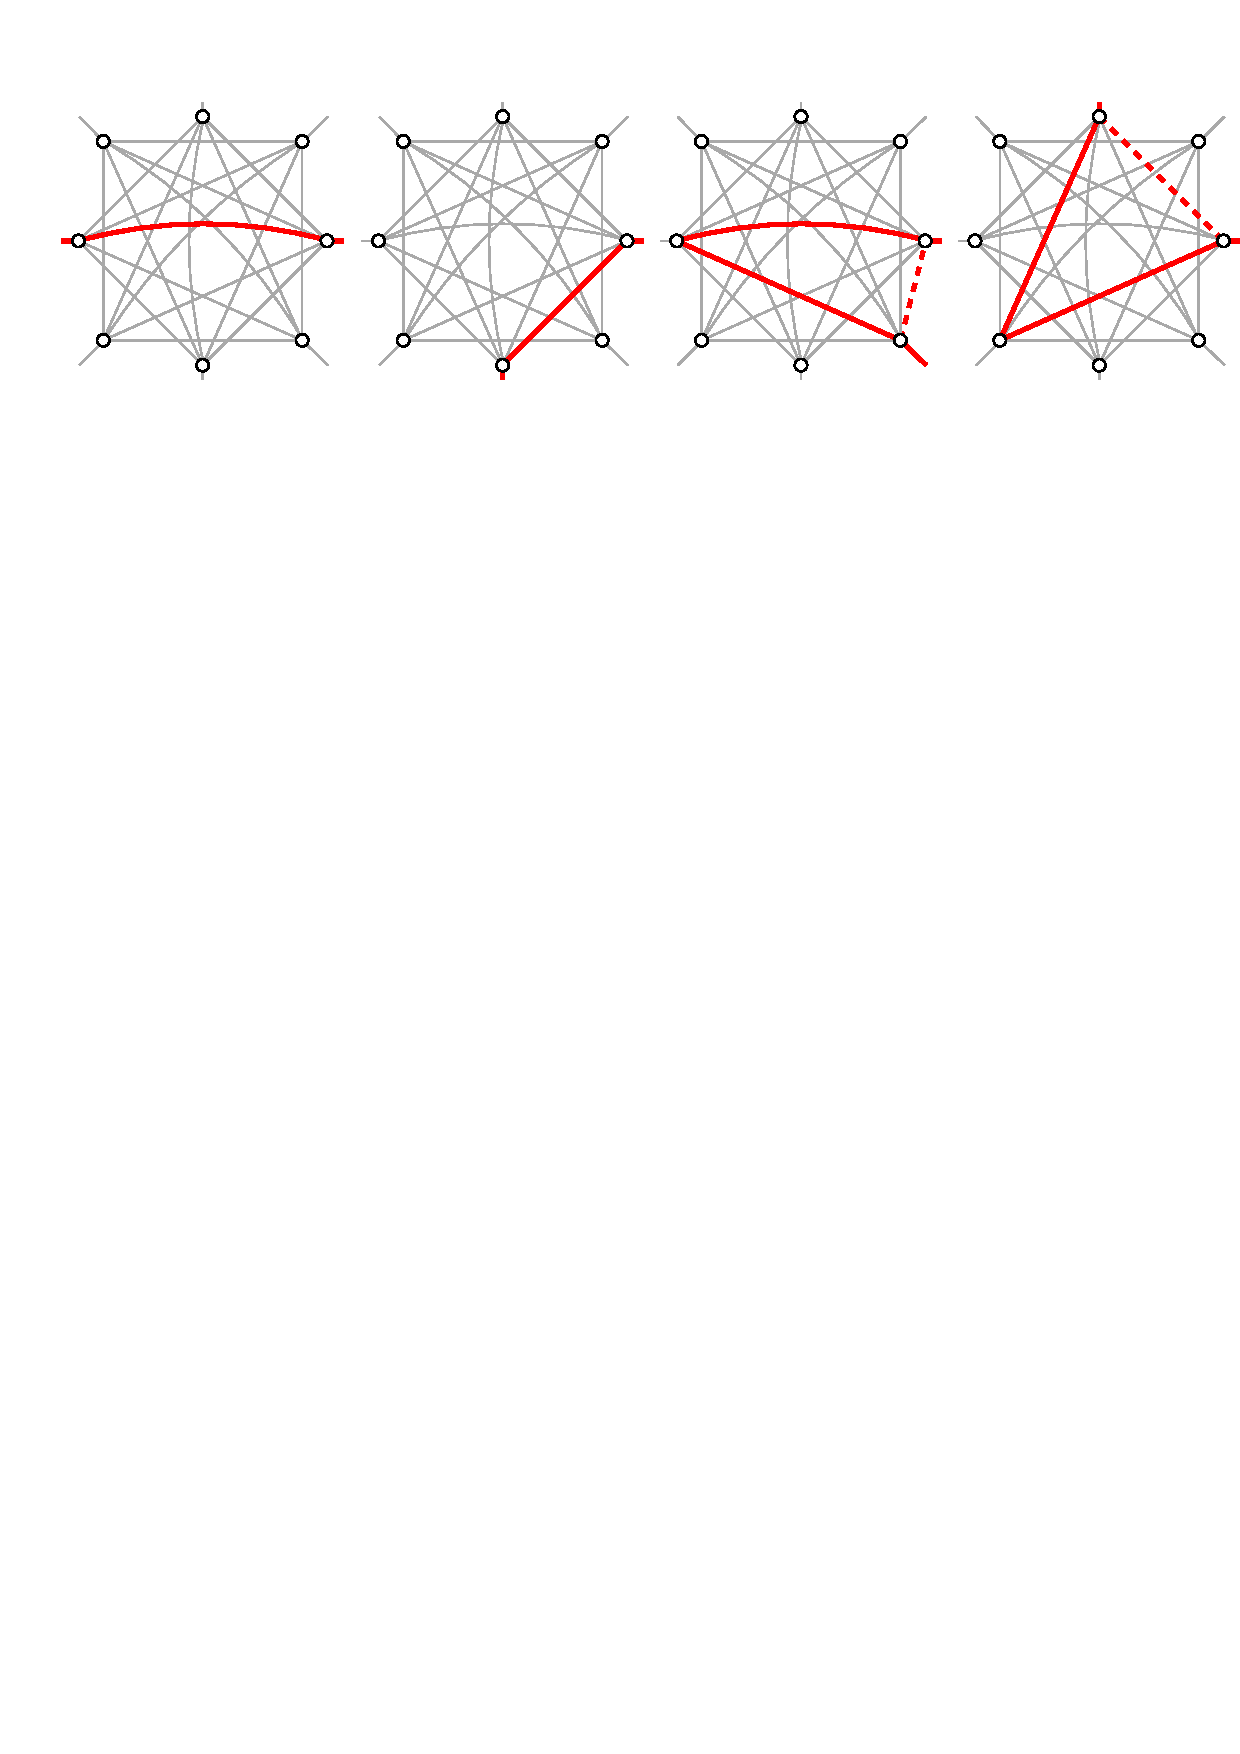
\includegraphics[width=0.9\textwidth]{figures/paths.pdf}}}$
	\caption{1. A $180^{\circ}$ pass through a node $\gv$. 2. A $90^{\circ}$ pass through $\psi$. 3. A $45^{\circ}$ pass through $\gv$ simulated by a $180^{\circ}$ and $135^{\circ}$ pass. 4. A $90^{\circ}$ pass through $\gv$ simulated by two $135^{\circ}$ passes. }
	\label{FIG:paths}
\end{figure*}
%
As both a $45^{\circ}$ port edge and a $90^{\circ}$ port edge may be substituted by cheaper edges, special care has to be applied to the modelling of the actual edge costs.
For example, a $45^{\circ}$ turn can be simulated by first passing $v_{x, y}$ on a $180^{\circ}$ port edge, and then again on a $135^{\circ}$ port edge (Fig.~\ref{FIG:paths}.3).
As $\gPturn{180} \leq \gPturn{135} \leq \gPturn{45}$, this path may be cheaper than $\gPturn{45}$, undermining our penalty system. 
Similarily, a $90^{\circ}$ degree turn can be simulated by two cheaper $135^{\circ}$ port edges (Fig.~\ref{FIG:paths}.4).

To prevent the shortcuts described above, we first introduce a constant $a \geq 0$ and set new port edge costs $\gPturnEdge{180}, ..., \gPturnEdge{45}$ as follows:
%
\begin{align}
	\gPturnEdge{180} &= a + \gPturn{180} = a \\
	\gPturnEdge{135} &= a + \gPturn{135} \\
	\gPturnEdge{90} &= a + \gPturn{90} \\
	\gPturnEdge{45} &= a + \gPturn{45}.
\end{align}
%
We choose $a$ in a way such that the following inequalities are fullfilled:
%
\begin{align}
	2a + 2\gPturn{135} &\geq a + \gPturn{90} \label{CONSTRS:sim90}\\
	2a + \gPturn{135} + \gPturn{90} &\geq a + \gPturn{45}\label{CONSTRS:sim45}.
\end{align}
Ineq.~(\ref{CONSTRS:sim90}) ensures that simulating a $90^{\circ}$ bend with two $135^{\circ}$ passes is never cheaper than $\gPturnEdge{90}$.
Ineq.~(\ref{CONSTRS:sim45}) ensures that simulating a $45^{\circ}$ bend with a $135^{\circ}$ pass and a $180^{\circ}$ pass is never cheaper than $\gPturnEdge{45}$.

The inequalities are fullfilled for $a = \gPturn{45} - \gPturn{135}$.

The shortest path $\gPathOcti$ from an original grid node $s = \gv_0$ to another original grid node $t=\gv_{n'}$ on our octilinear grid graph will now consist of \emph{two} nodes for each original grid node: for the start and end node, the original grid node and a single port node appear in the path.
For pass-through nodes, a port node for arriving at and a port node for leaving the original grid node appears (w.l.o.g., we ignore the case where a turn edge is replaced by two turn costs with similar cost, as this does neither affect the final path on the grid graph, nor the cost of that path).

This shortest path $\gPathOcti = (\gv_0, \gv_1, ..., \gv_{n'})$ thus always describes a path $\gPath = (\gv^*_0, \gv^*_2, \gv^*_4, ..., \gv^*_{n})$ on the original grid graph with $|p| = n = |p'| / 2 = n' / 2$ and has the cost
%
\begin{align}
	\gPcostOcti{\gPathOcti} = 2 \gSinkcost + \left(n - 1\right) \cdot \gHopcost + \sum_{i=1}^{n - 1} a + t\left(\gv^*_{2i - 2}, \gv^*_{2i+2}\right)\label{EQ:cost}.
\end{align}
%
To get rid of the constant offset $a$, we set $c_{135} = 1$, $c_{90} = 1.5$ and $c_{45} = 2$, which means $a = 1$.
If we then set the cost of a single grid edge $\gHopcost = 1 = a$ and set the actual grid edge costs to $\gHopcostOcti = \gHopcost - a = 0$, we can rewrite Eq.~\ref{EQ:cost} as  
%
\begin{align}
	\gPcostOcti{\gPathOcti} &= 2 c_s +  \left(n - 1\right) \cdot \gHopcostOcti + \sum_{i=1}^{n - 1} \gHopcost + t\left(\gv^*_{2i - 2}, \gv^*_{2i+2}\right) \\
	     &= 2 c_s + \left(n - 2\right) \cdot \gHopcost + \sum_{i=1}^{n - 1} t \left(\gv^*_{2i - 2}, \gv^*_{2i+2}\right) \\
	     &= 2 c_s + \gPcost{\gPath} - \gHopcost = \gPcost{\gPath} + 2 \gSinkcost - 1.
\end{align}
%
As the shortest path $p'$ thus minimizes $c(p) + 2 \gSinkcost - 1$, it also minimizes $\gPcost(\gPath)$.

\section{Optimal Solution via ILP}

Using the octilinear grid graph, we now define the problem of finding the optimal metro-map drawing on the grid defined by $\gG$ like this: find grid nodes for each input node and non-intersecting shortest paths in the grid graph between the grid nodes for adjacent input nodes.
The ordering of paths at grid node candidates should match the original embedding.
%The shortest paths in the grid than form an octilinear drawing of $\gG$ in which the original embedding is preserved.
This solution should minimizes the sum of (1) all shortest path costs, (2) the distance between the grid position of a station and its original position, and (3) the line bend penalties at stations (which are not covered by the path costs on $\gG$).

We first describe how to solve this problem exactly using an Integer Linear Program (ILP).
To encode the direction of a path from $\gv_s$ to $\gv_t$ in the ILP, we first model each undirected grid edge $\{\gv, \gv'\}$ as a pair of directed edges $(\gv, \gv')$ and $(\gv', \gv)$.
%This transforms our undirected grid graph into an equivalent directed grid graph.
To get unique start and end nodes for the shortest path calculations, we also treat each input edge $\ie = \{s, t\}$ now as a directed edge $(s, t)$.
As the shortest paths in $\gG$ are symmetric, it does not matter whether we chose $\ie = (s, t)$ or $\ie = (t, s)$.

To be able to later retrieve the placement of stations, we add binary decision variables $\gvused{\iv}{\gv}$ for each input node $\iv$ and grid node $\gv \in \gV^g$ which should be 1 of $\iv$ was assigned to $\gv$, or 0 otherwise.
We denote this grid node as $\gv_\iv$.
$\gvused{\iv}{\gv}$ is added to the objective function with the distance between the original position of $\iv$ and the position induced by $\gv$ as a coefficient.
To be able to deduce the course of the shortest paths, we define binary variables $\geused{\ie}{\ge}$ for each input edge $\ie$ and each grid edge $\ge$ which should be 1 if $\ge$ is used in path for $e$, or 0 otherwise.
$\geused{\ie}{\ge}$ is added to the objective function with the cost of grid edge $\ge$ as a coefficient.

\subsection{Station Placement}

To ensure that each input node $\iv \in \iV$ is assigned to exactly one grid node $\ggv{x}{y} \in \gV^g$, we add the following constraint:
%
\begin{equation}
  \forall \iv \in \iV: \sum_{\gv \in \gV^g} \gvused{\iv}{\gv} = 1. \label{EQ:onegvperiv}
\end{equation}
%
As a grid node can either be assigned a single input station, used as a pass-through for a single input edge, or be not used at all, we additionally add the following constraint:
%
\begin{equation}
  \forall \gv \in \gV^g: \sum_{\iv \in \iV} \gvused{\iv}{\gv} + \sum_{\ie \in \iE} \sum_{\ge \in \gE^b_\gv} \geused{\ie}{\ge} \geq 1, \label{EQ:singleuse}
\end{equation}
%
where $\gE^b_\gv$ is the set of bend edges adjacent to $\psi$. 
If an input station is assigned to $\gv$, the first sum is already 1, forbidding further use.
Similarily, if $\gv$ is used as a pass-through, it cannot be assigned to an input station node or be used as a pass-through by another path.
Note that Equation~\ref{EQ:singleuse} also enforces that a grid edge $\ge$ can only be used by a single path, as a second path using $\ge$ would have to either arrive or pass through a grid node that is already used by the other path on $\ge$.

\subsection{Edge Continuity}

To globally compute the shortest paths on $\gG$ between all adjacent input nodes, we build on the standard formulation of the shortest path problem as a Linear Program.
We first have to make sure that edges assigned to the shortest path from $\gv_s$ to $\gv_t$ are connected with the following constraints (where $e = (s, t)$):
%
\newcommand\Psum[1]{\sum_{\makebox[0pt]{$\scriptstyle#1$}}}
%
\begin{align}
	&\forall \ie \in \iE\ \forall \gv \in \gV^p:& \Psum{\ge \in \text{out}(\gv)} \geused{\ie}{\ge} - \Psum{\ge \in \text{in}(\gv)} \geused{\ie}{\ge}& = 0, \label{EQ:cont_port} \\
	&\forall \ie \in \iE\ \forall \gv \in \gV^g:& x_{t\psi} - 2x_{s\psi} + \Psum{\ge \in \text{out}(\gv)} 2\geused{\ie}{\ge} - &\Psum{\ge \in \text{in}(\gv)} \geused{\ie}{\ge} = 0. \label{EQ:cont_grid}
\end{align}
%
Equation~\ref{EQ:cont_port} guarantees that the number of outgoing and incoming edges at each port node is the same.
% This ensures a continuous path between $\gv_s$ and $\gv_t$.
%
Equation~\ref{EQ:cont_grid} handles $\gv_s$ and $\gv_t$.
Here we count an outgoing edge twice, which means that the grid node could only make up for an outgoing edge with two incoming edges.
This, however, would mean that our shortest path split somewhere, which is prevented by Equation~\ref{EQ:cont_port}.
The only way to fullfill the constraint is thus for $\gv$ to be the source node $\gv_s$ for the input edge.
Similarily, the only way to counter an incoming edge is for $\gv$ to be the target node $\gv_t$ for the input edge.

\subsection{Preservation of Embedding}

To preserve the input embedding, it is enough to guarantee that no two paths in $\gG$ intersect and that the circular ordering of adjacent edges is the same as in the input graph.
Equation~\ref{EQ:singleuse} already prevents paths crossing at grid nodes.
To prevent crossings at intersecting grid edges, we define $\gE^d$ as the set of diagonal grid edges and say that for $\ge \in \gE^d$, $\ge^{\times} \in \gE^d$ is the diagonal edge crossing $\ge$. 
We then add the following constraint:
%
\begin{equation}
  \forall \ge \in \gE^d: \Psum{\ie \in \iE} \geused{\ie}{\ge} + \geused{\ie}{\ge^{\times}} \leq 1. \label{EQ:crossing}
\end{equation}
%
To ensure that the edge ordering at nodes remains the same, we would first like to have a variable $\dir{\iv}{\ie} \in \{0, ..., 7\}$ which tells us the direction of input edge $\ie$ at adjacent input node $\iv$ in the final octilinear drawing.
To get the desired assignments, we add the following constraints:
%
\begin{align}
  \forall \ie = (s, t) \in \gE&: \sum_{\gv \in \gV^g} \sum_{p = 1}^7 p x_{e(\psi,  \psi^p)} - \dir{s}{e} = 0\label{EQ:dirfrom} \\
  \forall \ie = (s, t) \in \gE&: \sum_{\gv \in \gV^g} \sum_{p = 1}^7 p x_{e(\psi^p, \psi)} - \dir{t}{e} = 0\label{EQ:dirto}
\end{align}
%
In Equation~\ref{EQ:dirfrom}, each outgoing sink edge $(\gv,  \gv^{p}), p \in {0, ..., 7}$ adds $p$ to the sum.
As Equations~\ref{EQ:cont_grid} and \ref{EQ:singleuse} ensures that only a single outgoing sink edge in the grid graph may be used by the path for an input edge, we can be sure that the left side of the equation always exactly equals the octilinear direction $0, ..., 7$ of $e = (s, t)$ at $s$.
The only way to fullfil the constraint is thus to set the value of $\dir{s}{e}$ to the octilinear direction.
Equation~\ref{EQ:dirfrom} is modelled equivalently for paths incoming at $t$.

To finally ensure that the edge ordering in the final drawing matches the input drawing, we apply a trick originally used in \cite{noellenburg}.
If $v_0, ..., v_p, ..., v_{\text{deg}(u) - 1}$ is the clockwise ordering of nodes adjacent to u in the original embedding, then $\dir{v}{(v, u_{p})} < \dir{v}{(v, u_{p + 1})}$ has to be true for all but one $p \in \{0, ..., \text{deg}(u) - 1\}$ in the final octilinear drawing.
This can be enforced with the following constraints, which we add for all  $u \in \iV$ with $\deg(u) > 2$:
%
\begin{align}
  \dir{v}{(v, u_{p + 1})} - \dir{v}{(v, u_{p})} + 8\beta_p(v) &\geq 1,\label{EQ:dirs}\\
  \sum_{p = 0}^{\deg(u)-1} \beta_p(v) &\geq 1\label{EQ:onedev}.
\end{align}
%
If $\dir{v}{(v, u_{p})} \not< \dir{v}{(v, u_{p + 1})}$, then $\dir{v}{(v, u_{p + 1})} - \dir{v}{(v, u_{p})} \leq 0$ and the only way to fullfill Equation~\ref{EQ:dirs} is to set $\beta_p(v)$ to 1.
Equation~\ref{EQ:onedev} ensures that this can only happen a single time.

\subsection{Avoiding Line Bends}

So far, our shortest paths only penalize line bends along paths.
We have to ensure that line bends at input nodes are equivalently penalized.
We would like to have binary variables telling us whether edges $e$ and $f$ in the input graph describe a $45^{\circ}$, $90^{\circ}$, $135^{\circ}$ or $180^{\circ}$ bend at their joint node in the final drawing.
%As $G$ is not a multigraph, this joint node is unique.

We first note that for two directional variables $\dir{u}{e}$ and $\dir{u}{f}$, $\dir{u}{e} - \dir{u}{f} \mod 8$ is either 1 or 7 for $45^\circ$ bends, 2 or 6 for $90^\circ$ bends, 3 or 5 for $135^\circ$ bends and 4 for $180^\circ$ bends.
As modulo cannot be used directly in an ILP, we use the following equivalent constraint for each pair $e, f$ of edges in the input graph adjacent at node $u$ and sharing a line:
%
\begin{equation} 
  0 \leq \dir{u}{e} - \dir{u}{f} + 8 \gamma_{ef} \leq 7 \label{EQ:dirneg}.
\end{equation}
%
%The auxiliary binary variable $\gamma_{ef}$ will be 1 if $\dir{u}{f} > \dir{u}{e}$.
%As both $\dir{u}{e}$ and $\dir{u}{f}$ are in the range $[1, 8]$ and as $\dir{u}{e} \neq \dir{u}{f}$ (per Eq.~\ref{EQ:singleuse})
We then have $\dir{u}{e} - \dir{u}{f} + 8 \gamma_{ef} = \dir{u}{e} - \dir{u}{f} \mod 8$, which we will denote by $\dirdiff{u}{f}$.
We now add binary decision variables $\bend{e}{f}{0}, ..., \bend{e}{f}{7}$ for each of the 8 possible values of $\dirdiff{u}{f}$ and the following constraint for each pair of adjacent input edges:
%
\begin{equation} 
  \dirdiff{e}{f} - \sum_{i = 0}^7 i\bend{e}{f}{i} = 0 \label{EQ:bendassign}.
\end{equation}
%
To make sure that only one of the bend variables is set to 1, we add the following constraint:
%
\begin{equation} 
  \sum_{i = 0}^7 i\bend{e}{f}{i} = 1 \label{EQ:bendsum}.
\end{equation}
%
Each of the 8 bend variables is then added to the objective function with its corresponding penalty.

\subsection{ILP Complexity}

For an $X \times Y$ grid, our octilinear grid graph has $\Theta(XY)$ edges and nodes.
For the station placement, we need ${\Theta}(|V|XY)$ variables.
Additionally, Equations~\ref{EQ:onegvperiv} and \ref{EQ:singleuse} add ${\Theta}(|V|XY)$ constraints.
For the shortest path calculations, we need ${\Theta}(|E|XY)$ variables and constraints.
For the preservement of the embedding, Equation~\ref{EQ:crossing} adds ${\Theta}(XY)$ constraints.
Equations~\ref{EQ:dirfrom} and \ref{EQ:dirto} add ${\Theta}(|E|)$ constraints.
Equations~\ref{EQ:dirs} and \ref{EQ:onedef} add ${\Theta}(|V|)$ constraints.
Finally, for avoiding line bends and input nodes, we add at most number of $8\times7$ auxiliary variables per input node (as there can be at most $8\times7$ edge pairings per input node in our octilinear setting) and at most $8^2\times7$ bend variables per input node.
Similarily, Equations~\ref{EQ:dirneg}, \ref{EQ:bendassign} and \ref{EQ:bendsum} all add at most $8\times7$ constraints per input node, so the overall number of constraints and variables for the line bend penalty at input nodes is ${\Theta}(|V|)$.
The total number of constraints and variables in our ILP is thus ${\Theta}(|E|XY + |V|XY)$.

\section{Approximative Solution}

Solution times for the ILP described in the previous section tend to get very big for complex input graphs. \TODO{how big?}
This section describes a method to solve the problem approximatively, based on iterative shortest-path calculations on the octilinear grid graph described in TODO.
Our method works as follows:
  (1) Order the edges of the input graph.
  (2) For each ordered input edge $e = \{u, v\}$, calculate the shortest path from a set of possible start nodes to a set of possible target nodes on the grid graph. If the grid node for $u$ or $v$ has already been settled, the corresponding node set has size 1. Paths already calculated act as obstacles.
  (3) If no initial drawing could be found, randomize the ordering and try again.
  (4) Optimize the initial drawing via a local search approach where individual nodes are moved to one of their 8 neighboring positions and adjacent edges re-routed.
  (5) Build the drawing from the shortest paths.

Each step is described in detail in this section.
In particular, we explain how line bends at input nodes can be optimized, how we preserve the initial input embedding and how the shortest path search on the grid graph can be sped up with an $A^*$ heuristic.

\subsection{Input Edge Ordering}

In addition to the standard degree $\deg(\iv)$ of an input node $\iv$, we define the line degree $\ldeg(\iv)$ of a node a node to be the number of (non-unique) lines on each adjacent edge.
We then build our initial input edge ordering $o = (e_0, e_1, ..., e_{|E|})$ as follows:
  (1) Mark all input nodes as unprocessed.
  (2) Take the unprocessed node $\iv$ with highest line degree $\ldeg(\iv)$ and mark it as dangling.
  (3) As long as there are dangling nodes, take the dangling node $\iv_d$ with highest line degree and add all adjacent edges $\{\iv_d, u_0\}, ..., \{\iv_d, u_k\}$ leading to an unprocessed node $u_i$ to the edge ordering $o$, where the $u_i$ are sorted in ascending order w.r.t $\ldeg(u_i)$. In other words, we add the edge going to the adjacent node of highest line degree first, then the edge with second highest line degree, and so on. Mark each $u_i$ as dangling, and $\iv_d$ as processed. 
  (4) If there are no dangling nodes anymore, but unprocessed nodes remain, then the input graph was disconnected. In this case, we start again at (2).

Figure TODO gives an example.

\subsection{Edge Routing and Station Placement}

With an initial edge ordering at hand, we can start routing each input edge $\ie_i = \{\iv, u\}$ through the octilinear grid graph.
To get unique source and target nodes, we again treat each undirected input edge as a directed edge $\ie_i = (s, t)$.
As the grid positions (and therefore the grid nodes) for $\iv$ and $u$ may be still unknown, we route between sets $S_g$ and $T_g$.
$S_g$ consists of candidate grid nodes for $s$, $T_g$ are candidate grid node for $t$.
As candidates, we use all grid nodes within a threshold distance $\hat d$ \TODO{other symbol for that} around the original position of the input node.
If both $s$ are $t$ are not settled yet, it may happen that $S_g$ and $T_g$ are not disjoint.
To prevent this, we build a local Voronoi diagram: we first define $ST = S_g \cup T_g$ and say that for each $\ggv{x}{y} \in ST$, $\ggv{x}{y}$ is placed in $S'_g$ if it is nearer to $s$ than $t$, or in $T'_g$ otherwise.

\TODO{sink edge costs}

After that, we calculate the set-to-set shortest path between $S_g$ and $T_g$ using a standard implementation of Dijkstra's algorithm (to find the shortest path out of a set of source nodes to a set of target nodes, it is enough to init all $\ggv{x}{y} \in S_g$ with distance 0 and abort the algorithm as soon as any $\ggv{x}{y} \in T_g$ is settled.)

\subsection{Preservation of Embedding}

\begin{figure}
  \centering
	$\vcenter{\hbox{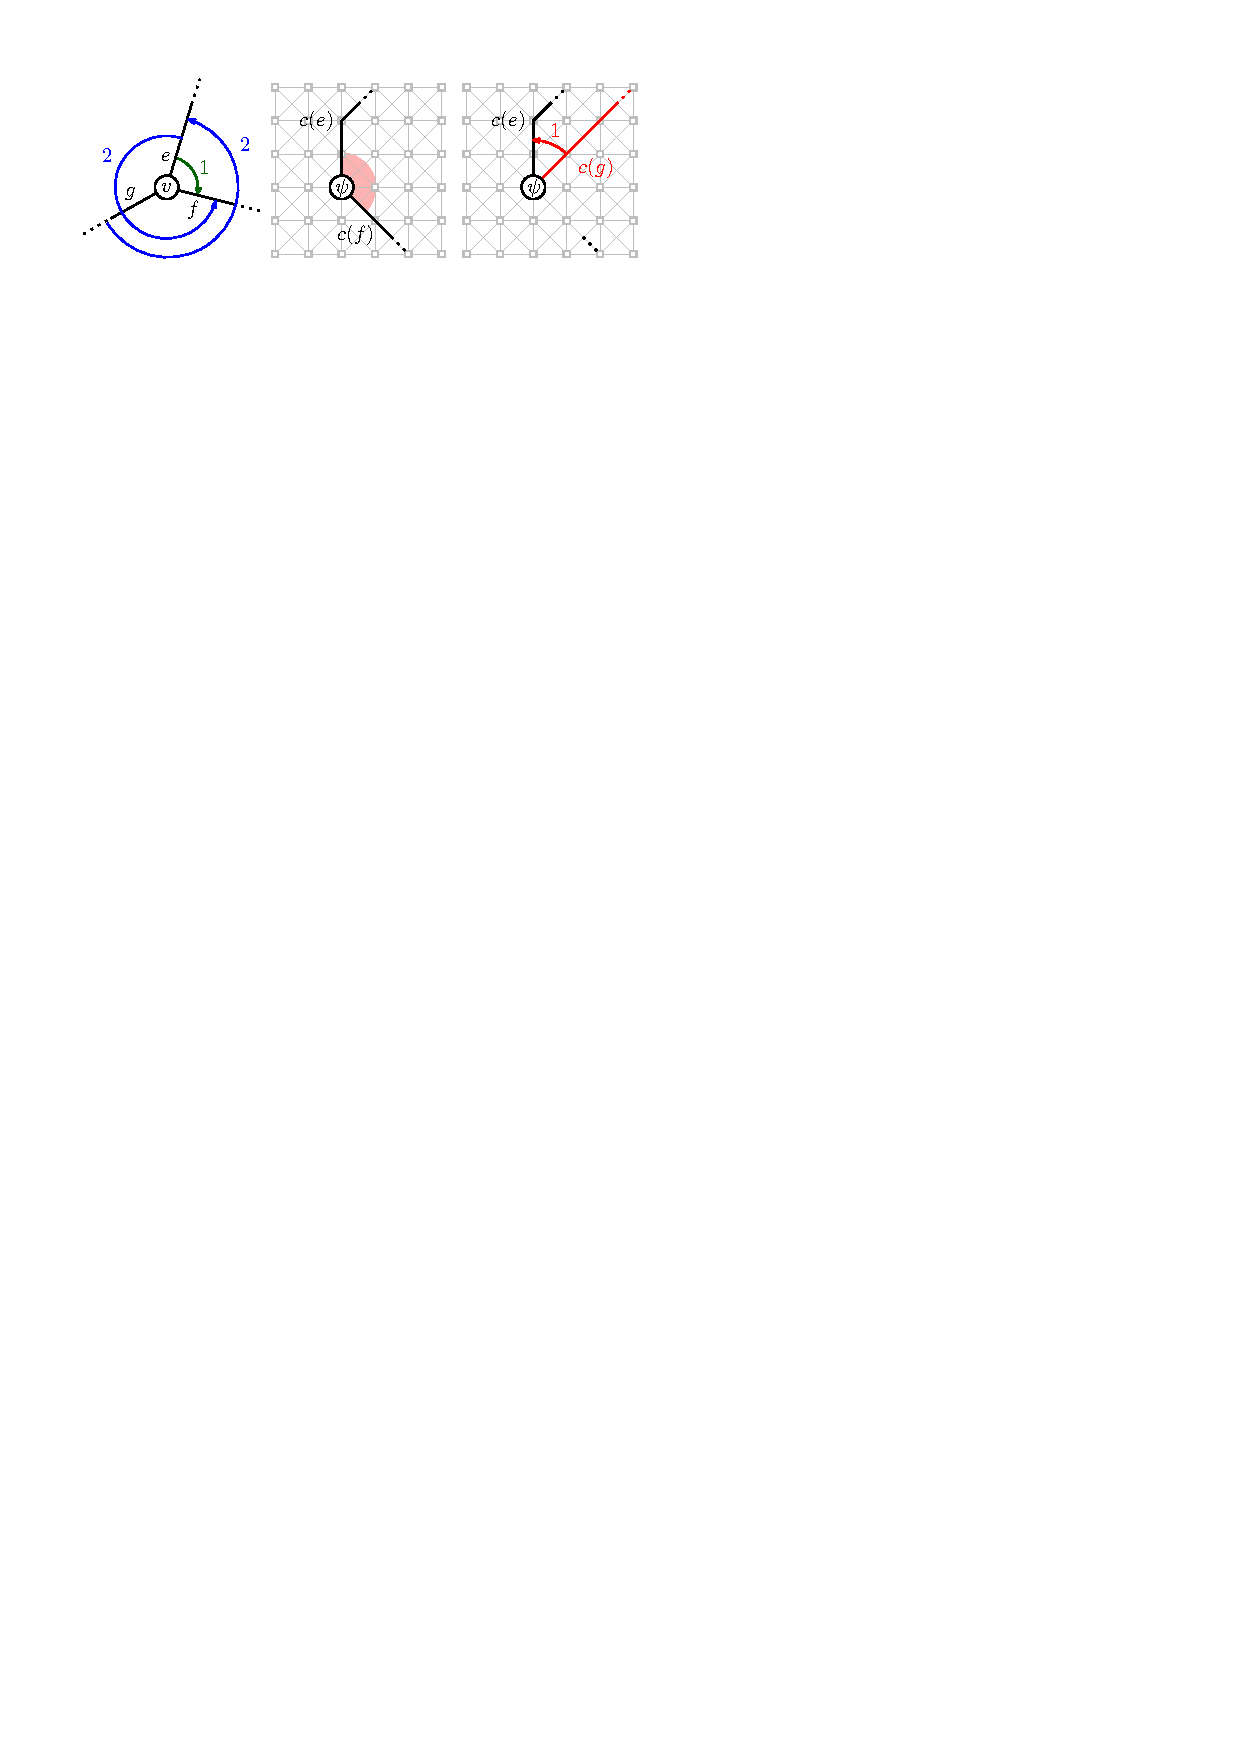
\includegraphics[width=0.479\textwidth]{figures/topoblock.pdf}}}$
	\caption{1. A $180^{\circ}$ pass through a node $\gv$. 2. A $90^{\circ}$ pass through $\psi$. 3. A $45^{\circ}$ pass through $\gv$ simulated by a $180^{\circ}$ and $135^{\circ}$ pass. 4. A $90^{\circ}$ pass through $\gv$ simulated by two $135^{\circ}$ passes. }
	\label{FIG:paths}
\end{figure}

The preserve the input embedding in our final drawing, we have to make sure that the shortest paths never cross each other, and that the initial circular ordering of edges at nodes is preserved.

To prevent paths crossing each other, we update our octilinear grid graph after each Dijkstra run.
Grid nodes that were used as nodes in the previously found shortest path are \emph{closed} by setting the cost of each adjacent turn edge to $\infty$.
If a closed node $\ggv{x}{y}$ was the source or target node for the previous path in $\Gamma$, it may later be used again as a source node for another input edge.
We therefore have to open it again in this case.

To prevent paths crossing each other at crossing diagonal edges in the grid graph, we additionally close for each diagonal grid edge used in the previously found path all crossing diagonal grid edges by setting their cost to $\infty$.

To preserve the circular edge ordering at nodes, we update the costs of adjacent sink edges for the grid node used for $s$, and the grid node used for $t$.
We consider Figure TODO.
In particular, we have to make sure that no 

\subsection{Avoiding Line Bends}

\subsection{Optimization via Local Search}

\subsection{Complexity}

\subsection{Speed-up Heuristic}

\section{Evaluation}

\subsection{Penalty Experiments}

\section{Conclusions}


\balancecolumns
\end{document}
